\UseRawInputEncoding % Add this line at the beginning

\documentclass{article}
\usepackage[utf8]{inputenc} % Assurer l'encodage UTF-8
\usepackage[T1]{fontenc}
\usepackage[french]{babel}
\usepackage{amsmath, amssymb}
\usepackage{graphicx}
\usepackage{microtype}
\usepackage{tikz}
\usetikzlibrary{intersections, calc}
\usepackage{pgfplots}
\pgfplotsset{compat=newest}
\usepackage{listings}
\usepackage{xcolor}
\usepackage{amsthm}
\usepackage{graphicx}
\usepackage{color}
\usepackage[margin=1in]{geometry}
% Define custom colors for code
\definecolor{codegreen}{rgb}{0,0.6,0}
\definecolor{codegray}{rgb}{0.5,0.5,0.5}
\definecolor{codepurple}{rgb}{0.58,0,0.82}
\definecolor{backcolour}{rgb}{0.95,0.95,0.92}
\usetikzlibrary{calc}
% Configure listings package
\lstdefinestyle{mystyle}{
    backgroundcolor=\color{backcolour},
    commentstyle=\color{codegreen},
    keywordstyle=\color{magenta},
    numberstyle=\tiny\color{codegray},
    stringstyle=\color{codepurple},
    basicstyle=\ttfamily\footnotesize,
    breakatwhitespace=false,
    breaklines=true,
    captionpos=b,
    keepspaces=true,
    numbers=left,
    numbersep=5pt,
    showspaces=false,
    showstringspaces=false,
    showtabs=false,
    tabsize=2
}
\lstset{style=mystyle}
\lstset{literate=%
{é}{{\'e}}{1}%
{è}{{\`e}}{1}%
{à}{{\`a}}{1}%
{ç}{{\c{c}}}{1}%
{œ}{{\oe}}{1}%
{ù}{{\`u}}{1}%
{É}{{\'E}}{1}%
{È}{{\`E}}{1}%
{À}{{\`A}}{1}%
{Ç}{{\c{C}}}{1}%
{Œ}{{\OE}}{1}%
{Ê}{{\^E}}{1}%
{ê}{{\^e}}{1}%
{î}{{\^i}}{1}%
{ô}{{\^o}}{1}%
{û}{{\^u}}{1}%
{ä}{{\"{a}}}1
{ë}{{\"{e}}}1
{ï}{{\"{i}}}1
{ö}{{\"{o}}}1
{ü}{{\"{u}}}1
{û}{{\^{u}}}1
{â}{{\^{a}}}1
{Â}{{\^{A}}}1
{Î}{{\^{I}}}1
}
% Additional settings for microtype and document formatting
\tolerance=2000
\emergencystretch=10pt
\newtheorem{lemma}{Lemme}
\newtheorem{remark}{Remarque}
\begin{document}

\title{Résolution d'équations non linéaires par la méthode de Newton}


\maketitle
\newpage
\tableofcontents
\newpage


\section{Rappel et Définitions}
\subsection{Fonction Holomorphe}
Soit $\Omega$ un domaine (ouvert non vide connexe) de $\mathbb{C}$. Une fonction $f : \Omega \to \mathbb{C}$ est C-dérivable en $z_0 \in \Omega$ si la limite
\[
\lim_{z \to z_0} \frac{f(z) - f(z_0)}{z - z_0} = \lim_{h \to 0} \frac{f(z_0 + h) - f(z_0)}{h}
\]
existe dans $\mathbb{C}$. On la note alors $f'(z_0)$ et on l’appelle la dérivée de $f$ en $z_0$. La fonction $f$ est holomorphe sur $\Omega$ si elle est C-dérivable en tout point de $\Omega$. Dans ce cas, la fonction $z \in \Omega \mapsto f'(z)$ est appelée dérivée de $f$.

Une fonction entière est une fonction holomorphe sur l’ensemble $\mathbb{C}$ tout entier.

Une fonction $f$ est holomorphe en $z_0$ si elle est holomorphe sur un voisinage de $z_0$.\\

\textbf{Notation:}
L’ensemble des fonctions holomorphes sur $\Omega$ sera noté $\Theta(\Omega)$.

\subsection{Points Singuliers (Singularité)}
Soit $f : \mathbb{C} \to \mathbb{C}$. $z_0$ est une singularité de $f$ s'il existe un voisinage $V$ de $z_0$ tel que $f$ soit holomorphe en tout point de $V$ sauf en $z_0$.

On considérera la forme générale de la série de Laurent de $f$ sur une couronne $C(z_0, r_1, r_2)$ $ 0 \leq r_1 < r_2$(la rendant holomorphe)  donnée par :

\[
f(z) = \sum_{m=1}^{+\infty} a_-m (z - z_0)^{-m} + \sum_{n=0}^{+\infty} a_n (z - z_0)^n
\]

Pour $z \in C(z_0, r_1, r_2)$.

On dit que $z_0$ est un pôle d'ordre $k$ de $f$ si pour tout $m > k$, $a_{-m} = 0$ et $a_{-k} \neq 0$.

\subsection{Fonction Méromorphe}
Une fonction $f$ est dite méromorphe sur le domaine $\Omega \subset \mathbb{C}$ si elle est une fonction $f : \Omega \to \mathbb{C}$ qui est holomorphe à l'exception de singularités isolées qui sont toutes des pôles pour $f$.

Autrement dit, s'il existe un ensemble $A \subset \Omega$ tel que :
\begin{itemize}
    \item[(a)] $A$ n'a pas de point d'accumulation dans $\Omega$,
    \item[(b)] $f \in \Theta(\Omega \setminus A)$,
    \item[(c)] chaque point de $A$ est un pôle pour $f$.
\end{itemize}
L'ensemble des singularités de $f$ est appelé l'ensemble polaire de $f$.

\textbf{Remarque}
\begin{itemize}
    \item Il est possible que $A = \emptyset$. Cela signifie que si nous notons $\mathcal{M}(\Omega)$ l'ensemble des fonctions méromorphes sur $\Omega$, on a : $\Theta(\Omega) \subset \mathcal{M}(\Omega)$.
    \item $A$ est au plus dénombrable puisque l'hypothèse (a) implique qu'aucune partie compacte de $\Omega$ ne contient une infinité de points de $A$.
\end{itemize}

\textbf{Exemple:} \\
La fonction 
\[
f(z) = \frac{g(z)}{(z - z_1)^{k_1}(z - z_2)^{k_2} \cdots (z - z_n)^{k_n}}
\]
où $g$ est une fonction holomorphe aux voisinages de $z_1, \ldots, z_n$ et non nulle en chacun de ces points est une fonction méromorphe sur $\mathbb{C}$.

La fonction $\tan(\pi z) = \frac{\sin(\pi z)}{\cos(\pi z)}$ est une fonction méromorphe sur $\mathbb{C}$. Elle n'a que des pôles simples en $z_k = \frac{1}{2} + k, k \in \mathbb{Z}$.

\subsection{Réseau de $ \mathbb{C}$ }
Un sous-groupe additif $\Omega \subset \mathbb{C}$ est un réseau si :
\begin{enumerate}
    \item $\Omega$ est discret,
    \item $\Omega$ engendre $\mathbb{C}$ sur $\mathbb{R}$.
\end{enumerate}

\subsection{Périodicités de fonctions Méromorphes }
\textbf{Définition 1.1} \quad Une fonction méromorphe \( f: \mathbb{C} \to \mathbb{C} \) est dite \textit{périodique de période} \( \tau \in \mathbb{C}^* \) si pour tout \( z \) dans \( \mathbb{C} \): 
\[ z + \tau \in \Omega \quad \text{et} \quad f(z + \tau) = f(z) \]


\textbf{Remarque 1.2} \quad Il n'y a pas unicité de la période d'une telle fonction, en effet, pour tout \( \lambda \) dans \(  \tau  \mathbb{Z} \), \( \lambda\) est une période de \( f \).


On note \( \Lambda_f \) l'ensemble des périodes de la fonction \( f \).

\textbf{Proposition 1.3} \quad Soit \( f \) une fonction méromorphe non constante, de trois choses l'une:
\begin{enumerate}
    \item \( \Lambda_f = \emptyset \)
    \item Il existe \( \tau_1 \in \mathbb{C}^* \) une période de \( f \) avec \( |\tau_1| \) minimal tel que \( \Lambda_f = \tau_1 \mathbb{Z}^* \)
    \item Il existe \( \tau_1, \tau_2 \in \mathbb{C}^* \) deux périodes de \( f \) tel que:
    \[
\frac{\tau_1}{\tau_2} \notin \mathbb{R} \quad \text{et} \quad \forall \tau \in \Lambda_f:  \exists! (n, m) \in \mathbb{Z}^2, \quad \tau = n\tau_1 + m\tau_2
\]
\end{enumerate}
Nous appellerons de telles périodes \( \tau_1 \) et \( \tau_2 \) des périodes fondamentales de \( f \).



\textbf{Proposition 1.4} \quad Toute fonction méromorphe avec trois périodes indépendantes est constante.


\textbf{Remarques 1.5}
\begin{itemize}
    \item[(i)] Le théorème nous dit en réalité que si nous sommes dans le 3ème cas: \( \Lambda_f = \tau_1 \mathbb{Z} + \tau_2 \mathbb{Z} \); \( \tau_1 \) et \( \tau_2 \) des périodes fondamentales de \( f \).
    \item[(ii)] Il n'y a pas unicité des périodes fondamentales de \( f \), par exemple, \( \pm \tau_1 \) et \( \pm \tau_2 \) sont aussi périodes fondamentales.
    \item[(iii)] Toute fonction vérifiant le 3ème cas est dite doublement périodique.
\end{itemize}

\begin{figure}[h]
    \centering
    \begin{tikzpicture}[scale=1.5]
        % Define the grid
        \foreach \x in {0,1,2,3,4,5}
        \foreach \y in {0,1,2,3}
        {
            \draw (\x,\y) -- (\x+1,\y); % horizontal lines
            \draw (\x,\y) -- (\x,\y+1); % vertical lines
        }
        
        % Add the last set of lines to complete the grid
        \foreach \y in {0,1,2,3}
        {
            \draw (6,\y) -- (6,\y+1);
        }
        \foreach \x in {0,1,2,3,4,5,6}
        {
            \draw (\x,4) -- (\x+1,4);
        }
        
        % Labels and specific vectors
        \draw[thick, red, ->] (3,2) -- node[below] {$\tau_1$} (4,2);
        \draw[thick, red, ->] (3,2) -- node[left] {$\tau_2$} (3,3);
    \end{tikzpicture}
    \caption{Illustration du 3ème cas}
    \end{figure}
    
    
\begin{lemma}[1.6]
Soit \( f \) une fonction périodique non constante, l'ensemble \( \Lambda_f \) ne contient pas de point d'accumulation, c'est un ensemble discret de \( \mathbb{C} \).
\end{lemma}

\textbf{Démonstration.}
On démontre ce lemme par l'absurde. Posons \( \alpha \in \Lambda_f \) un point d'accumulation et soit \( P \) l'ensemble des pôles de \( f \). Il existe une suite \( (\tau_n) \) de \( \Lambda_f \) telle que \( (\tau_n) \) converge vers \( \alpha \) tel que pour tout \( i \neq j \), \( \tau_i \neq \tau_j \). Soit \( z_0 \in \mathbb{C}\setminus P \), \( z_0 + \alpha \in \mathbb{C}\setminus P \) car \( \alpha \in \Lambda_f \), par continuité de la fonction \( f \) et périodicité : 
\[
f(z_0 + \alpha) = \lim_{n \to \infty} f(z_0 + \tau_n) = f(z_0)
\]
Ainsi, \( z_0 + \alpha \) est un zéro non isolé de la fonction méromorphe \( f - f(z_0) \). Ainsi par le théorème des zéros isolés, \( f - f(z_0) \) est identiquement nulle, donc \( f \equiv f(z_0) \), ce qui est impossible car \( f \) est supposée non constante.

\begin{remark}[1.7]
    Pour tout \( A \) non vide tel que \( A \subseteq \Lambda_f \). Alors, il existe \( \tilde{r} \in A \) tel que :
    \[ |\tilde{r}| = \inf\{|r|: r \in A\} \]
    En effet, \( \{r : |r| \in A\} \) est une partie non vide minorée par 0 sans point d'accumulation. Elle admet donc un minimum.

\end{remark}

\textbf{Démonstration de la proposition.}

Si \( \Lambda_f = \{0\} \), nous sommes dans le 1\textsuperscript{er} cas. On suppose donc maintenant que \( \Lambda_f \neq \{0\} \).

D'après la remarque précédente, on sait qu'il existe \( r_1 \in \Lambda_f \) tel que
\[
|r_1| = \inf\{|r|, r \in \Lambda_f\}
\]
Posons \( B = r_1\mathbb{Z} \). Il est immédiat que \( B \subseteq \Lambda_f \).

Si \( B = \Lambda_f \), nous sommes dans le 2\textsuperscript{ème} cas, en revanche si \( B \neq \Lambda_f \), il faut montrer que nous sommes dans le 3\textsuperscript{ème} cas.

En utilisant à nouveau la remarque pour \( \Lambda_f/B \), il existe \( r_2 \in \Lambda_f/B \) tel que
\[
|r_2| = \inf\{|r|, r \in \Lambda_f/B\}
\]

Alors \( \lambda \in \mathbb{R}\setminus\mathbb{Z} \), car \( \tau_2 \in \Lambda_f/B \), et de plus \( \tau_2 - \lambda\tau_1 = (\lambda - 1)\tau_1 \in \Lambda_f \), avec \( \lambda - 1 \neq 0 \); ce qui est impossible d'après la définition de \( \tau_1 \).
\begin{itemize}
    \item Montrons pour commencer que \( \frac{\tau_1}{\tau_2} \notin \mathbb{R} \). Supposons par l'absurde qu'il existe \( \lambda \in \mathbb{R} \) tel que \( \tau_2 = \lambda\tau_1 \).
    Alors \( \lambda \in \mathbb{R} \setminus \mathbb{Z} \), car \( \tau_2 \in \Lambda_f \setminus B \) et de plus  \[
        \tau_2 - \lfloor \lambda \rfloor \tau_1 = (\lambda - \lfloor \lambda \rfloor) \tau_1 \in \Lambda_f, \quad \text{avec} \quad \lambda - \lfloor \lambda \rfloor \in ]0; 1[
        \],ce qui est impossible d'après la définition de \( \tau_1 \).
    
    \item Montrons maintenant que toute période \( \tau \) de \( \Lambda_f \) peut s'écrire de manière unique sous la forme
    \[
    \tau = n\tau_1 + m\tau_2, \quad n, m \in \mathbb{Z}.
    \]
\end{itemize}

En effet, puisque \(\frac{\tau_1}{\tau_2} \notin \mathbb{R}\), \((\tau_1, \tau_2)\) forme une base de \(\mathbb{C}\) en tant que \(\mathbb{R}\) espace vectoriel; ce qui entraîne l'existence de deux scalaires uniques \(\lambda_1\) et \(\lambda_2\) tels que \(\tau = \lambda_1 \tau_1 + \lambda_2 \tau_2\). De plus, il existe deux entiers \(n_1\) et \(n_2\) tels que \(|\lambda_1 - n_1| \leq \frac{1}{2}\) et \(|\lambda_2 - n_2| \leq \frac{1}{2}\).

Ainsi :
\[
(\lambda_1 - n_1)\tau_1 + (\lambda_2 - n_2)\tau_2 = \tau - n_1\tau_1 - n_2\tau_2 \in \Lambda_f
\]

Par conséquent:
\begin{enumerate}
    \item Si \(\lambda_1 - n_1 = \lambda_2 - n_2 = 0\), alors \(\tau = n_1\tau_1 + n_2\tau_2\).
    \item Si \(\lambda_1 - n_1 = 0\) et \(\lambda_2 - n_2 \neq 0\), alors \((\lambda_2 - n_2)\tau_2 \in \Lambda_f\) et \(\left|(\lambda_2 - n_2)\tau_2\right| \leq |\tau_2|\).\\
    Donc, par définition de \(\tau_2\), \((\lambda_2 - n_2)\tau_2 \in B\), d'où l'existence d'un \(n \in \mathbb{Z}\) tel que \(\tau = n_1\tau_1 + n_2\tau_2\).
    \item Le cas \(\lambda_1 - n_1 \neq 0\) et \(\lambda_2 - n_2 = 0\) est impossible car \((\lambda_1 - n_1)\tau_1\ \in \Lambda_f\) et \(\left|(\lambda_1 - n_1)\tau_1\right| < |\tau_1|\), ce qui contredit la définition de \(\tau_1\).
    \item Si \((\lambda_1 - n_1)(\lambda_2 - n_2) \neq 0\), on a, puisque \(\frac{\tau_1}{\tau_2} \notin \mathbb{R}\):
    \[
    \left|\tau - n_1\tau_1 - n_2\tau_2\right| \leq \left|(\lambda_1 - n_1)\tau_1\right| + \left|(\lambda_2 - n_2)\tau_2\right| \leq \frac{1}{2}\left(|\tau_1| + |\tau_2|\right) \leq |\tau_2|
    \]
    Donc, par définition de \(\tau_2\), \(\tau -n_1\tau_1 - n_2\tau_2 \in B\), d'où l'existence d'un \(n \in \mathbb{Z}\) tel que \(\tau = n_1\tau_1 + n_2\tau_2\).
\end{enumerate}



\section{Fonctions élliptiques}
\textbf{Définitions de fonction elliptique: \\}


On appelle \textit{fonction elliptique} toute fonction méromorphe dans $\mathbb{C}$ non constante doublement périodique.


Dans cette section, nous allons nous intéresser aux résultats principaux des fonctions elliptiques avant d'expliciter des exemples dans la section suivante.


\textbf{Définitions d'un parallélogramme: \\}
Soient $ a \in \mathbb{C}  \ et \  \omega_1, \omega_2 \in \mathbb{C}^{*}$, on appelle \textit{parallélogramme} dans $\mathbb{C}$ l'ensemble :
\[
\mathcal{P}_{a}{(\omega_1, \omega_2)} = \{ a + \alpha \omega_1 + \beta \omega_2 \mid 0 \leq \alpha, \beta < 1 \}
\]
Dans le cas où $f$ est une fonction elliptique de périodes fondamentales $\omega_1$ et $\omega_2$ et $a=0$, on parlera d'un \textit{parallélogramme fondamental} de $f$. On le notera dans la suite $\mathcal{P}{(\omega_1, \omega_2)}$.


\begin{center}
\begin{tikzpicture}
    \coordinate (O) at (0,0);
    \coordinate (A) at (2,0);
    \coordinate (B) at (1,2);
    \coordinate (C) at ($(A) + (B)$);
    
    \draw[thick] (O) -- (A) -- (C) -- (B) -- cycle;
    \draw[dashed] (O) -- (B);
    \draw[dashed] (A) -- (C);
    
    \node at (-0.2,-0.2) {$a$};
    \node at (2.2,-0.2) {$a +\omega_1$};
    \node at (1,2.2) {$a +\omega_2$};
    \node at (3.2,2.2) {$a +\omega_1 + \omega_2$};
\end{tikzpicture}
\end{center}
\begin{center}
\textit{Illustration d'un parallélogramme issu de $a$.}
\end{center}

\textbf{Théorème de Liouville \\}

    Toute fonction $f$ elliptique holomorphe sur $\mathbb{C}$ est constante.


\textbf{Lemme: \\}

    Soient $\omega_1, \omega_2 \in \mathbb{C}^{*}$ tels que $\frac{\omega_1}{\omega_2} \notin \mathbb{R}$. Alors pour tout $z$ dans $\mathbb{C}$, on peut associer un unique $z' \in \mathcal{P}_{a}{(\omega_1, \omega_2)}$ et deux uniques $n, m \in \mathbb{Z}$ tels que $z = z' + n \omega_1 + m \omega_2$.


\textbf{Démonstration.}

En effet, $\frac{\omega_1}{\omega_2} \notin \mathbb{R}$ donc $\{ \omega_1, \omega_2 \}$ est une base de $\mathbb{C}$ en tant que $\mathbb{R}$ espace vectoriel, ce qui entraîne l'existence de deux scalaires uniques $\alpha, \beta \in \mathbb{R}$ tels que :
\[
z - a = \alpha \omega_1 + \beta \omega_2 = (\alpha - \lfloor \alpha \rfloor) \omega_1 + (\beta - \lfloor \beta \rfloor) \omega_2 + \lfloor \alpha \rfloor \omega_1 + \lfloor \beta \rfloor \omega_2
\]
\[
    (\alpha - \lfloor \alpha \rfloor), (\beta - \lfloor \beta \rfloor)  \in [0, 1]
\]

Donc on a bien montré l'existence d'une telle décomposition, il faut désormais montrer l'unicité. Pour cela, supposons que :
\[
z_1 + n_1 \omega_1 + m_1 \omega_2 = z = z_2 + n_2 \omega_1 + m_2 \omega_2
\]
et donc
\[
z_1 - z_2 = (n_2 - n_1) \omega_1 + (m_2 - m_1) \omega_2
\]
De plus, $z_1, z_2 \in \mathcal{P}_{a}(\omega_1, \omega_2)$, donc il existe $r, s \in  ]-1, 1[$ tels que $z_2 - z_1 = r \omega_1 + s \omega_2$

Par unicité de la décomposition dans la base ${\left\{ \omega_1, \omega_2\right\}}$ on en déduit :
\[
\begin{cases}
r = n_1 - n_2 \in \mathbb{Z} \\
s = m_1 - m_2 \in \mathbb{Z}
\end{cases}
\implies
\begin{cases}
r = 0 \\
s = 0
\end{cases}
\quad \text{car le seul entier entre -1 et 1 est 0}
\]

D'où l'unicité.

\textbf{Remarque 2.5}
Grâce à ce lemme, nous pouvons en déduire l'égalité suivante :
\[
\mathbb{C} = \bigcup_{\gamma \in \Lambda_{f}} P_{\alpha + \gamma} (\omega_1, \omega_2)
\]
\begin{figure}[h]
    \centering
    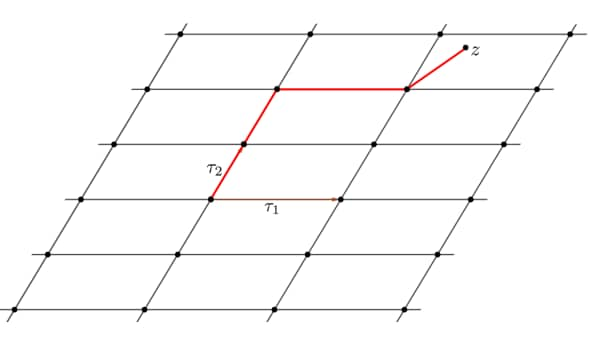
\includegraphics[width=0.6\textwidth]{lemme.jpeg}
    \caption{Illustration du \textit{lemme} 2.4 et de l'\textit{égalité} précédente}
\end{figure}



\subsection{Démonstration du théorème 2.3}

Soit $\mathcal{P}(\omega_1, \omega_2)$ un parallélogramme fondamental de $f$.

La fonction $f$ étant holomorphe sur $\mathbb{C}$, elle est donc continue et ainsi bornée sur $\partial \mathcal{P}(\omega_1, \omega_2)$, et par le principe du maximum, $f$ est bornée sur $\mathcal{P}(\omega_1, \omega_2)$.

Ainsi, d'après le lemme 2.4, tout nombre complexe $z$ peut s'écrire sous la forme :
\[
z = z' + n \omega_1 + m \omega_2 \quad \text{avec} \quad z' \in \mathcal{P}(\omega_1, \omega_2), \quad n, m \in \mathbb{Z}
\]
On en déduit donc 
\[
\sup_{z \in \mathbb{C}} |f(z)| = \sup_{z' \in \mathcal{P}(\omega_1, \omega_2)} |f(z')| < +\infty
\]
La fonction $f$ est donc bornée et entière, donc constante par le théorème de Liouville.

\subsection{Ordre d'une fonction elliptique}

Soit $z \in \mathbb{C}$. D'après le lemme 2.4, il existe $z' \in \mathcal{P}(\omega_1, \omega_2)$ et $n, m \in \mathbb{Z}$ tel que $z = z' + n \omega_1 + m \omega_2$. Vient alors :

\textbf{Proposition 2.6}
$z \in \mathbb{C}$ est un zéro ou un pôle d'ordre $p$ d'une fonction elliptique $f$ si et seulement si $z'$ est respectivement un zéro ou un pôle d'ordre $p$.

\section*{Démonstration}

Si $z$ est un pôle d'ordre $p$, par la caractérisation des pôles il existe $c$ tel que l'on ait :
\[
\lim_{h \to 0} h^p f(z + h) = c \iff \lim_{h \to 0} h^p f(\zeta + n\omega_1 + m\omega_2 + h) = c
\]
\[
\iff \lim_{h \to 0} h^p f(\zeta + h) = c
\]
\[
\iff \zeta \text{ est un pôle d'ordre } p \text{ de } f
\]
ce qui est un pôle d'ordre $p$ de $f$.

Si $z$ est un zéro d'ordre $p$. Remarquons que si $f$ est elliptique, $\frac{1}{f}$ est aussi elliptique ($\mathbb{C}$ est connexe donc $\mathcal{M}(\mathbb{C})$ est un corps, $\frac{1}{f}$ est donc méromorphe), ainsi on a :

$z$ est un zéro d'ordre $p$ de $f \iff \zeta$ est un pôle d'ordre $p$ de $\frac{1}{f}$ 
\[
\iff \zeta \text{ est un pôle d'ordre } p \text{ de } \frac{1}{f}
\]
\[
\iff \zeta \text{ est un zéro d'ordre } p \text{ de } f
\]

\textbf{Théorème 2.7}
Toute fonction elliptique $f$ possède au moins un pôle dans $P(\omega_1, \omega_2)$.


\section*{Démonstration}

Par l'absurde, si $f$ ne possède aucun pôle dans $P(\omega_1, \omega_2)$. Par la proposition 2.6, $f$ ne possède aucun pôle dans $\mathbb{C}$, ainsi $f$ est entière. Ainsi, $f$ est une constante, ce qui est une contradiction.

\textbf{Proposition 2.8}
Le nombre fini de pôles (compté avec multiplicité) d'une fonction elliptique $f$ dans un de ses parallélogrammes fondamental $P(\omega_1, \omega_2)$ est appelé l'ordre de $f$.


\section*{Démonstration}

Pour que cette définition ait un sens, il faut montrer que le nombre de pôles (compté avec multiplicité), est indépendant de la paire de périodes fondamentales.

Soient $(\omega_1, \omega_2)$ et $(\omega'_1, \omega'_2)$ deux paires de périodes fondamentales de $f$. Désignons $A$ et $B$ respectivement les pôles de $f$ dans $P(\omega_1, \omega_2)$ et $P(\omega'_1, \omega'_2)$.

D'après le \textbf{Théorème 2.7} et le \textbf{lemme 2.4}, $A$ et $B$ sont non vides et finis.
\[
j: A \rightarrow B
\]
\[
z \mapsto \zeta  
\]
\[
    \text{avec} \quad z \mapsto \zeta + n\omega'_1 + m\omega'_2, \quad \zeta \in B \quad \text{et} \quad n,m \in \mathbb{Z}.
    \]  
Cette fonction est bien définie par unicité de la décomposition de $z$ démontré dans le \textbf{lemme 2.4}. Il suffirait alors de montrer que $j$ est bijective pour obtenir le résultat voulu.

Soit \( z_1, z_2 \in A \) tel que \( j(z_1) = j(z_2) \). Alors, \( z_1 - z_2 \in \Lambda_f \) et il existe, puisque \( (\omega_1, \omega_2) \) est une paire de période fondamentale et de ce fait forme une base de \( \mathbb{C} \) en tant que \( \mathbb{R} \) espace vectoriel, deux scalaires \( r \) et \( s \) tels que :
\[
z_1 - z_2 = r\omega_1 + s\omega_2
\]
Comme de plus \( z_1, z_2 \in P(\omega_1, \omega_2) \) et \( z_1 - z_2 \in \Lambda_f \); \( -1 < r, s < 1, r, s \in \mathbb{Z} \).

Par conséquent, par l'unicité d'une telle décomposition, \( r = s = 0 \) et on a bien \( z_1 = z_2 \).

Soit \( c \in B \). Alors, il existe \( z \in A \) et \( n, m \in \mathbb{Z} \) tels que :
\[
c = z + n\omega_1 + m\omega_2.
\]
Ainsi, \( (\omega_1, \omega_2) \) étant une paire de périodes fondamentales de \( f \), il existe \( p_1, p_2, q_1, q_2 \in \mathbb{Z} \) tels que :
\[
z = (c -n\omega_1 + m\omega_2) = c  -n(p_1\omega'_1 + q_1\omega'_2) - m(p_2\omega'_1 + q_2\omega'_2) = (c + (-n p_1 - m p_2)\omega'_1 + (-n\ q_1 - m q_2)\omega'_2)
\]
D'où, \( j(z) = c \)

La fonction \( j \) est donc bijective, \( A \) et \( B \) étants finis, on en déduit que \( |A| = |B| \).

\textbf{Proposition 2.9} L'ordre d'une fonction elliptique est supérieur ou égal à 2

\textbf{Lemme 2.10} La somme des résidus des pôles de \( f \) dans un de ses parallélogrammes \( P_a(\tau_1,\tau_2) \) est nulle.

\textbf{Démonstration.}
Soient \( \{b_1, \ldots, b_n \}\) les $n$ pôles distincts de \( f \) contenus dans \( P_a(\tau_1, \tau_2) \).
Supposons pour commencer que \( \{b_1, \ldots, b_n\} \cap \partial P(\tau_1, \tau_2) = \emptyset \).
En supposant le bord \( P_a(\tau_1, \tau_2) \) orienté positivement, on a d'après le théorème des résidus :
\[
-2\pi i \sum_{j=1}^n \text{Res}(f, b_j) = \int_{\partial P(\tau_1,\tau_2)} f(z) \, dz
\]
\begin{tikzpicture}[scale=1.5]
    % Define the points
    \coordinate (A) at (0,0);
    \coordinate (B) at (2,0);
    \coordinate (C) at (3,1.5);
    \coordinate (D) at (1,1.5);

    % Draw the parallelogram
    \draw[thick] (A) -- (B) -- (C) -- (D) -- cycle;

    % Draw small red arrows in the middle of each side to indicate direction
    \draw[-latex, red, thick, shorten >=1mm, shorten <=1mm] ($(A)!0.5!(B)$) -- (A);
    \draw[-latex, red, thick, shorten >=1mm, shorten <=1mm] ($(B)!0.5!(C)$) -- (B);
    \draw[-latex, red, thick, shorten >=1mm, shorten <=1mm] ($(C)!0.5!(D)$) -- (C);
    \draw[-latex, red, thick, shorten >=1mm, shorten <=1mm] ($(D)!0.5!(A)$) -- (D);

    % Label the sides with gamma
    \node[red] at ($(A)!0.5!(B)!0.3cm!90:(B)$) {$\gamma_4$};
    \node[red] at ($(B)!0.5!(C)!0.3cm!90:(C)$) {$\gamma_3$};
    \node[red] at ($(C)!0.5!(D)!0.3cm!90:(D)$) {$\gamma_2$};
    \node[red] at ($(D)!0.5!(A)!0.3cm!90:(A)$) {$\gamma_1$};

    % Label the vertices
    \node at (A) [below left] {$a$};
    \node at (B) [below right] {$a +\tau_1$};
    \node at (C) [above right] {$a +\tau_1 + \tau_2$};
    \node at (D) [above left] {$a +\tau_2$};
\end{tikzpicture}

Ainsi :
\[
\int_{\partial P(\tau_1,\tau_2)} f(z) \, dz = \int_{\gamma_1} f(z) \, dz + \int_{\gamma_2} f(z) \, dz + \int_{\gamma_3} f(z) \, dz + \int_{\gamma_4} f(z) \, dz 
\]
\[
= \tau_1 \int_0^1 f(\tau_1 t) \, dt + \tau_2 \int_0^1 f(\tau_1 + \tau_2 t) \, dt - \tau_1 \int_0^1 f(\tau_2 + \tau_1 t) \, dt - \tau_2 \int_0^1 f(\tau_2 t) \, dt
\]
\[
= \tau_1 \int_0^1 f(\tau_1 t) \, dt + \tau_2 \int_0^1 f(\tau_2 t) \, dt - \tau_1 \int_0^1 f(\tau_1 t) \, dt - \tau_2 \int_0^1 f(\tau_2 t) \, dt
\]
\[
= 0
\]
Supposons désormais qu'au moins un des pôles \( b_j \) se trouve sur le bord de \( P(\tau_1, \tau_2) \).

Les pôles étant isolés, il existe \( \alpha \in \mathbb{C}^* \) tel que sur le bord du parallélogramme fondamental translaté 
\[
P_\alpha = \{ \zeta + \alpha, \zeta \in P(\tau_1, \tau_2)\}
\]
il n’y a aucun pôle de la fonction \( f \) mais que son intérieur contienne tous les pôles de \( f \) contenus dans \( P(\tau_1, \tau_2) \) et seulement ceux-ci.

En effet, soit \( S \) l'ensemble des pôles de \( f \), \( S \cap P_\alpha \) est fini, donc il existe \(  \tilde{r} \in [0, 1] \) tel que :
\[
\{\tilde{r}\tau_1 + s\tau_2, s \in [0, 1]\} \cap S = \emptyset
\]
De même, il existe \( \tilde{s} \in [0, 1] \) tel que 
\[
\{r\tau_1 + \tilde{s}\tau_2, r \in [0, 1]\} \cap S = \emptyset
\]
On pose alors \( \alpha = \tilde{r}\tau_1 + \tilde{s}\tau_2 \), ainsi :

\begin{align*}
    \partial P_\alpha = & \left\{ (\tilde{r}+r)\tau_1 + \tilde{s}\tau_2, r \in [0, 1[ \right\} \cup \\
                        & \left\{ (\tilde{s}+ s)\tau_2 + \tilde{r}\tau_1, s \in [0, 1[ \right\} \cup \\
                        & \left\{ (\tilde{r} + r)\tau_1 + (\tilde{s} + 1)\tau_2, r \in [0, 1[ \right\} \cup \\
                        & \left\{ (\tilde{r} + 1)\tau_1 + (\tilde{s} + s)\tau_2, s \in [0, 1[ \right\} \cup \\
                        & \left\{ (\tilde{r} + 1)\tau_1 + (\tilde{s} + 1)\tau_2 \right\}
    \end{align*}
n'intersecte pas \( S \) par \( \Lambda_f \) périodicité de \( f \).

Ainsi par un calcul identique au précédent appliqué au parallélogramme \( P_\alpha \), on obtient que la somme des résidus est nulle.


\textbf{Démonstration de la proposition 2.9.}

Supposons par l'absurde que \( o(f) < 2 \).

Si \( o(f) = 0 \), \( f \) ne possède pas de pôle et est donc holomorphe. Or toute fonction elliptique holomorphe est constante, ce qui contredit l'hypothèse.

Si \( o(f) = 1 \). Posons \( p \) l'unique pôle (simple) de \( f \).

Au voisinage de \( p \) on peut alors écrire \( f(z) = \frac{\lambda}{z - p} + g(z) \), avec \( g \) une fonction holomorphe.

Mais alors, \( \text{Res}(f, p) = \lambda \), d'après le lemme 2.10 on a donc \( \lambda = 0 \), donc \( f \) est holomorphe; finalement \( f \) est constante contrairement à l'hypothèse.

\textbf{Théorème 2.11}

Toute fonction elliptique d'ordre \( m \) possède exactement \( m \) zéros (comptés avec multiplicité) dans \( P_{\alpha}(\tau_1, \tau_2) \), \( a \in \mathbb{C} \).

\textbf{Lemme 2.12}

Soit \( f \) une fonction elliptique \( \Lambda_f \)-périodique, \( f' \) est une fonction elliptique \( \Lambda_f\)-périodique.

\textbf{Démonstration.}

Pour tout \( z \in \mathbb{C} \), \( \lambda \in \Lambda_f \) \( f: f(z + \lambda) = f(z) \)

Ainsi en dérivant cette égalité on obtient : \( f'(z + \lambda) = f'(z) \)

La dérivée d'une fonction méromorphe est aussi une fonction méromorphe, on en déduit alors que \( f' \) est une fonction 
elliptique \( \Lambda_f \)-périodique.

\textbf{Démonstration du théorème.}

Supposons pour commencer qu'il n'y ait ni zéro ni pôle de \( f \) sur \( \partial P(\tau_1, \tau_2) \).

En supposant \( \partial P(\tau_1, \tau_2) \) orienté positivement, d'après le théorème de l'indice :
\[
2\pi i(\mu - \nu) = \int_{\partial P(\tau_1, \tau_2)} \frac{f'(z)}{f(z)} \, dz
\]

\[
= \tau_1  \int_0^1 \frac{f'(\tau_1 t)}{f(\tau_1 t)} \, dt + \tau_2 \int_0^1 \frac{f'(\tau_1 + \tau_2 t)}{f(\tau_1 + \tau_2 t)} \, dt - \tau_1 \int_0^1 \frac{f'(\tau_2 + \tau_1 t)}{f(\tau_2 + \tau_1 t)} \, dt - \tau_2 \int_0^1 \frac{f'(\tau_2 t)}{f(\tau_2 t)} \, dt 
\]
\[
= \tau_1  \int_0^1 \frac{f'(\tau_1 t)}{f(\tau_1 t)} \, dt + \tau_2\int_0^1 \frac{f'( \tau_2 t)}{f( \tau_2 t)} \, dt - \tau_1\int_0^1 \frac{f'( \tau_1 t)}{f( \tau_1 t)} \, dt - \tau_2\int_0^1 \frac{f'(\tau_2 t)}{f(\tau_2 t)} \, dt
\]
\[
= 0
\]
Où \( \mu \) et \( \nu \) sont respectivement le nombre de zéros et de pôles (comptés avec multiplicité) de la fonction \( f \) dans \( P(\tau_1, \tau_2) \).

Supposons à présent qu'au moins un des pôles ou un des zéros de \( f \) se trouve sur le bord \( \partial P(\tau_1, \tau_2) \). Les pôles étant isolés, il existe \( \alpha \in \mathbb{C}^* \) tel que sur le bord du parallélogramme fondamental translaté
\[
P_\alpha = \{\zeta + \alpha, \zeta \in P(\tau_1, \tau_2)\}
\]
il n'y a aucun pôle de la fonction \( f \) mais que son intérieur contienne tous les pôles de \( f \) contenus dans \( P(\tau_1, \tau_2) \) et seulement ceux-ci.

Ainsi par un calcul identique au précédent appliqué au parallélogramme \( P_\alpha(\tau_1, \tau_2) \), on montre que dans \( P_\alpha(\tau_1, \tau_2) \), donc dans \( P(\tau_1, \tau_2) \), la fonction \( f \) a le même nombre de zéros que de pôles (comptés avec multiplicité).

\textbf{Remarque 2.13}

Nous avons démontré au passage que l'ensemble des fonctions elliptiques de périodes \( \tau_1 \) et \( \tau_2 \) est stable par dérivation et que c'est un corps pour l'addition et la multiplication, mais nous ne savons pas encore s'il existe des fonctions elliptiques non triviales.

\textbf{Corollaire 2.14}

Soit \( f \) une fonction elliptique d'ordre \( m \). Alors pour tout \( \omega \in \mathbb{C} \), l'équation \( f(z) = \omega \) admet exactement \( m \) solutions (comptées avec multiplicité).

\textbf{Proposition 2.15}

Soit \( f \) une fonction elliptique. Alors, si \( a_1, \ldots, a_p \) sont les zéros distincts d'ordres respectifs \( n_1, \ldots, n_p \), et \( b_1, \ldots, b_q \) les pôles distincts d'ordre respectifs \( m_1, \ldots, m_q \) de la fonction \( f \) dans \( P_{\alpha}(\tau_1, \tau_2) \), \( a \in \mathbb{C} \), il existe deux entiers \( n \) et \( m \) tels que :
\[
\sum_{j=1}^p n_j a_j - \sum_{j=1}^q m_j b_j = n\tau_1 + m\tau_2
\]

\textbf{Démonstration.}

Supposons pour commencer qu'il n'y a ni zéros ni pôles de \( f \) sur \( \partial P(\tau_1, \tau_2) \). En supposant \( \partial P(\tau_1, \tau_2) \) orienté positivement, d'après le théorème des résidus :
\[
\frac{1}{2\pi i} \int_{\partial P(\tau_1, \tau_2)} z\frac{f'(z)}{f(z)} \, dz = \sum_{j=1}^p \text{Res}_{a_j} \left( Id\frac{f'}{f} \right) + \sum_{j=1}^q \text{Res}_{b_j} \left( Id\frac{f'}{f} \right)
\]

\textit{$a_j$, étant un zéro d'ordre $n_j$ de $f$, il existe $\delta_j > 0$ et $g_j \in H(B(a_j, \delta_j))$ tel que $  \forall z \in B(a_j, \delta_j): f(z) = (z - a_j)^{n_j} g_j(z)$ et $g_j(z) \neq 0$.}

Et donc, on a
\[
\frac{z f'(z)}{f(z)} = n_j + \frac{n_j a_j}{z - a_j} +   z  \frac{ g'_j(z)}{g_j(z)}
\]

D'où
\[
\text{Res}_{a_j} \left(  Id\frac{f'}{f} \right) = n_j a_j
\]

\textit{$b_j$, étant un pôle d'ordre $m_j$ de $f$, il existe $\rho_j > 0$ et $h_j \in H(B(b_j, \rho_j))$ tel que $ \forall z \in B(b_j, \rho_j) : f(z) = (z - b_j)^{-\rho_j} h_j(z)$ et $h_j(z) \neq 0$.}

Et donc, on a
\[
\frac{z f'(z)}{f(z)} = -m_j + \frac{-m_j b_j }{z - b_j} + z\frac{ h'_j(z)}{h_j(z)}
\]

D'où
\[
\text{Res}_{b_j} \left( Id\frac{f'}{f} \right) = -m_j b_j
\]

D'autre part, en revenant à la définition de l'intégrale curviligne, on a :

\begin{align*}
    \int_{\partial P(\tau_1,\tau_2)} \frac{f'(z)}{f(z)} \, dz &= \tau_1 \int_0^1 \tau_1 t \frac{f'(\tau_1 t)}{f(\tau_1 t)} \, dt + \\
    &\quad \tau_2 \int_0^1 (\tau_1 + \tau_2 t) \frac{f'(\tau_1 + \tau_2 t)}{f(\tau_1 + \tau_2 t)} \, dt - \\
    &\quad \tau_1 \int_0^1 (\tau_1 t + \tau_2) \frac{f'(\tau_1 t + \tau_2)}{f(\tau_1 + \tau_2)} \, dt - \\
    &\quad \tau_2 \int_0^1 \tau_2 t \frac{f'(\tau_2 t)}{f(\tau_2 t)} \, dt
    \end{align*}
\[
= \tau_1 \int_0^1 \tau_2\frac{f'(\tau_2 t)}{f(\tau_2 t)} \, dt - \tau_2 \int_0^1 \tau_1\frac{f'(\tau_1 t)}{f(\tau_1 t)} \, dt
\]
Montrons désormais que pour \( j = 1, 2 \):
\[
\int_0^1 \tau_j\frac{f'(\tau_j t)}{f(\tau_j t)} \, dt = k_j 2\pi i, \quad k_j \in \mathbb{Z}
\]
Pour cela, posons pour \( s \in [0,1] \): \( u_j(s) = f(\tau_j s)e^{-v_j(s)} \) où \( v_j(s) = \int_0^s \frac{f'(\tau_j t)}{f(\tau_j t)} \, dt \)
Ainsi, pour tout \( s \in [0, 1] \) on a :
\[
u_j'(s) = \tau_j f'(\tau_j s)e^{-v_j(s)} - \tau_j \frac{f'(\tau_j s)}{f(\tau_j s)} f(\tau_j s)e^{-v_j(s)} = 0
\]

Puis, grâce à la continuité de la fonction \( u \), pour tout \( s \in [0,1] \): \( u_j(s) = f(0) \)

Par conséquent,
\[
f(0) = u_j(1) = f(\tau_j)e^{-v_j(1)} = f(0)e^{-v_j(1)}
\]

et donc
\[
v_j(1) = \int_0^1 \tau_j\frac{f'(\tau_j t)}{f(\tau_j t)} \, dt = k_j 2\pi i, \quad k_j \in \mathbb{Z}
\]

En résumé,
\[
\sum_{j=1}^p n_j a_j - \sum_{j=1}^q m_j b_j = k_2\tau_1 - k_1\tau_2
\]

et en prenant \( n = k_2 \) et \( m = -k_1 \), on obtient le résultat.

Supposons à présent qu'au moins un des pôles ou un des zéros de \( f \) se trouve sur le bord \( \partial P(\tau_1, \tau_2) \). Les pôles étant isolés, il existe \( \alpha \in \mathbb{C}^* \) tel que sur le bord du parallélogramme fondamental translaté
\[
P_\alpha = \{\zeta + \alpha, \zeta \in P(\tau_1, \tau_2)\}
\]
il n'y ai aucun pôle de la fonction \( f \) mais que son intérieur contienne tous les pôles de \( f \) contenus dans \( P(\tau_1, \tau_2) \) et seulement ceux-ci.

Ainsi par un calcul identique au précédent appliqué au parallélogramme \( P_\alpha \), on peut conclure.

\section{Fonctions elliptiques de Weierstrass}
En mathématiques, les fonctions de Weierstrass sont des fonctions spéciales d'une variable complexe qui sont reliées à la fonction elliptique de Weierstrass $\wp(z)$.

\subsection{Fonctions $\wp(z)$ de Weierstrass}
Dans le chapitre précédent, nous avons vu de nombreux résultats sur les fonctions elliptiques. Il est très aisé de construire des fonctions ne possédant qu'une seule période, cependant, il est beaucoup plus compliqué de construire des fonctions (non triviales) admettant deux périodes fondamentales distinctes. Dans cette partie nous allons traiter l'exemple de la fonction $\wp$ de Weierstrass. Après avoir construit cette fonction, nous montrerons que toute fonction elliptique de même période que $\wp$ est une fonction rationnelle de $\wp$ et $\wp'$.

\subsubsection{Définition de la fonction $\wp$ de Weierstrass.}

Soient $\tau_1, \tau_2 \in \mathbb{C}^*$ tels que $\frac{\tau_1}{\tau_2} \notin \mathbb{R}$ fixes et posons
\[
\forall k \in \mathbb{N} : T_k = \{(n,m) \in \mathbb{Z}^2 \mid \max(|n|,|m|) = k\}
\]
Tous les $T_k$ sont symétriques par rapport à l'origine. Autrement dit,
\[
(n,m) \in T_k \iff (-n,-m) \in T_k
\]

\begin{figure}[h]
    \centering
    \begin{tikzpicture}[scale=1]
        % Grid lines
        \draw[step=1cm, gray, very thin] (-3.5,-3.5) grid (3.5,3.5);
        
        % T_3
        \fill[red!10] (-3,-3) rectangle (3,3);
        
        % T_2
        \fill[red!30] (-2,-2) rectangle (2,2);
        
        % T_1
        \fill[red!50] (-1,-1) rectangle (1,1);
        
        % Axes
        \draw[thick,->] (-3.5,0) -- (3.5,0) node[right] {$x$};
        \draw[thick,->] (0,-3.5) -- (0,3.5) node[above] {$y$};
        
        % Labels
        \node at (0,0) [below right, fill=white] {$T_1$};
        \node at (1,1) [below right, fill=white] {$T_2$};
        \node at (2,2) [below right, fill=white] {$T_3$};
        
        % Origin
        \fill[black] (0,0) circle (2pt) node[below left] {0};
    \end{tikzpicture}
    \caption{Illustration de \( T_k \) pour \( k=1,2,3 \)}
    \label{fig:Tk}
\end{figure}

Posons de plus :
\[
\forall n, m \in \mathbb{Z} : \sigma_{n, m} = n\tau_1 + m\tau_2
\]
\[
A = \{\sigma_{n, m}, n, m \in \mathbb{Z}\} \text{ et } A' = A \setminus \{0\}
\]
A définit un réseau symétrique par rapport à l'origine.

\textbf{Proposition / Définition 3.1}

Étant donné un réseau \( A \), on lui associe une fonction notée \( \wp_A \), où s'il n'y a pas de confusion à craindre, et définie sur \( \mathbb{C}/A \) par
\[
    \wp_A(z) = \frac{1}{z^2} + \sum_{\gamma \in A'} \left( \frac{1}{(z - \gamma)^2} - \frac{1}{\gamma^2} \right)
\]
Cette fonction est appelée fonction \( \wp \) de Weierstrass.

\begin{figure}
    \centering
    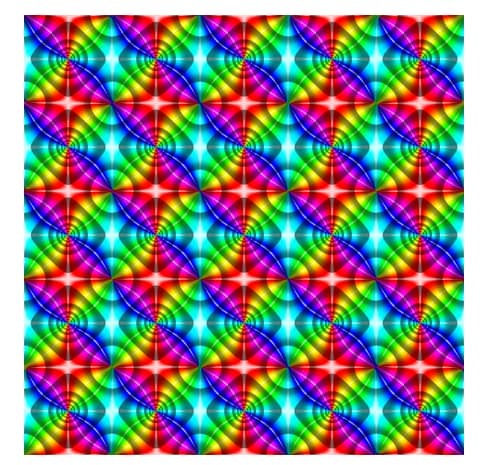
\includegraphics[width=\linewidth]{weierstrass_function.jpeg}
    \caption{Tracé de la fonction $\wp$ de Weierstrass par coloriage de domaine.}
\end{figure}


\textbf{Proposition 3.2}

La fonction \( \wp \) est méromorphe dans \( \mathbb{C} \). Plus particulièrement :
\begin{enumerate}
    \item \( \wp' \in H\left( \mathbb{C}/A \right)\) et \( \wp'(z) = -2 \sum_{\gamma \in A} \frac{1}{(z - \gamma)^3} \)
    \item Tous les points du réseau \( A \) sont des pôles doubles de \( \wp \) de résidu 0
\end{enumerate}

Pour montrer cette proposition ainsi que la bonne définition de \(\wp\), nous allons d'abord démontrer deux lemmes :

\textbf{Lemme 3.3}

Pour tout \(k \in \mathbb{N}^*\):
\[
\sum_{(n,m) \in T_k} \frac{1}{|\sigma_{n,m}|^3} \leq \frac{8}{\delta^3 k^2}
\]
où \(\delta = \min \{|\sigma_{n,m}|, (n,m) \in T_k\}\).

\textit{Démonstration.}

On a pour tout \(k > 0\):
\[
|T_k| = |\{(n,m) \in \mathbb{Z}^2, \max(|n|,|m|) \leq k\}| - |\{(n,m) \in \mathbb{Z}^2, \max(|n|,|m|) \leq k-1\}| = (2k+1)^2 - (2k-1)^2 = 8k
\]
\(T_k\) contient donc \(8k\) points.

Ensuite, pour tout \((n,m) \in T_k\): \(|\sigma_{n,m}| \geq k\delta\). En effet, supposons sans perte de généralité \(|\tau_1| \geq |\tau_2|\) \\
Nécessairement, \(\delta = |\sigma_{0,1}|\). Ainsi on a :
\[
|n\tau_1 + m\tau_2| \geq \max(|n|,|m|)\delta = k\delta
\]
On a alors immédiatement :
\[
\sum_{(n,m) \in T_k} \frac{1}{|\sigma_{n,m}|^3} \leq \sum_{(n,m) \in T_k} \frac{1}{(k\delta)^3} \leq\frac{8}{\delta^3 k^2}
\]

\textbf{Lemme 3.4}

Pour tout \(\omega \in \Lambda\), la suite \((\Psi_{\omega, p})\) définie par
\[
\Psi_{\omega, p}(z) = \sum_{(n,m) \in T_k, \sigma_{n,m} \neq \omega} \left( \frac{1}{(z - \sigma_{n,m})^2} - \frac{1}{\sigma_{n,m}^2} \right)
\]
est uniformément convergente sur tout compact \(K \subset \mathbb{C} \setminus (\Lambda^{*} \setminus \omega)\).\\


\textbf{Démonstration.}

Soit \(K\) un compact, il existe un nombre \(r > 0\) tel que \(K \subset B(0,r)\). Ainsi, puisque pour tout \(z \in K\) et tout \(\sigma_{n,m}\), \(|\sigma_{n,m}| \geq 2r\) :
\[
\left| \frac{1}{(z - \sigma_{n,m})^2} - \frac{1}{\sigma_{n,m}^2} \right| = \left| \frac{\sigma_{n,m}^2 - (z^2 - 2z\sigma_{n,m} + \sigma_{n,m}^2)}{\sigma_{n,m}^2 (z - \sigma_{n,m})^2} \right|
\]
\[
= \left| \frac{z(z - 2\sigma_{n,m})}{\sigma_{n,m}^2 (z - \sigma_{n,m})^2} \right|
\]
\[
= \frac{|z| \left| 2 - \frac{z}{\sigma_{n,m}} \right|}{|\sigma_{n,m}|^3 \left| 1 - \frac{z}{\sigma_{n,m}} \right|^2} 
\]
\[
< \frac{10r}{|\sigma_{n,m}|^3}
\]

On obtient ainsi, d'après le lemme précédent, que pour tout couple d'entier \( j > l > \frac{2r}{\delta} \):
\[
\sup_{z \in K} | \Psi_{w_{i},j}(z) - \Psi_{w_{i},l}(z) | \leq \sup_{z \in K} \left| \sum_{k=l+1}^{j} \sum_{(n,m) \in T_k, \sigma_{n,m} \neq 0} \left( \frac{1}{(z - \sigma_{n,m})^2} - \frac{1}{\sigma_{n,m}^2} \right) \right|
\]
\[
\leq 10r \sum_{k=l+1}^{j} \sum_{(n,m) \in T_k} \frac{1}{|\sigma_{n,m}|^3}
\]
\[
\leq \frac{80r}{\delta^3} \sum_{k=l+1}^{j} \frac{1}{k^2}
\]
Par conséquent, \((\Psi_{p,n})\) est une suite de Cauchy sur \(K\) pour \(||\cdot||_{\infty}\), elle est donc uniformément convergente sur \(K\).

Nous pouvons désormais démontrer la proposition 3.2.

\textbf{Démonstration.}

1. Pour montrer que la fonction \( \wp \) est bien définie sur \( \mathbb{C}/A \), on écrit :

\[
p(t) = \frac{1}{z^2} + \sum_{\gamma \in A'} \left( \frac{1}{(z - \gamma)^2} - \frac{1}{\gamma^2} \right)
\]
\[
= \frac{1}{z^2} + \lim_{p \to \infty} \Psi_{0,p}(z)
\]
Ensuite, d'après le théorème de Weierstrass et le lemme 3.4, la fonction
\[
\Psi_{0}(z) = \lim_{p \to \infty} \Psi_{0,p}
\]
est holomorphe dans \( \mathbb{C}/A' \) et
\[
\Psi'_{0}(z) = \lim_{p \to \infty} \sum_{k=1}^{p} \left( \sum_{(n,m) \in T_k} \left( \frac{1}{(z - \sigma_{n,m})^2} - \frac{1}{\sigma_{n,m}^2} \right)' \right)
\]
\[
= \sum_{k=1}^{ + \infty} \left( \sum_{(n,m) \in T_k} \left( -\frac{2}{(z - \sigma_{n,m})^2} \right) \right)
\]
\[
= -2 \sum_{\gamma \in A} \frac{1}{(z - \gamma)^3}
\]
D'où
\[
\wp \in H( \mathbb{C}/A) \quad \text{et} \quad \wp'(z) = -\frac{2}{(z)^3} + \Psi_0'(z) = -2 \sum_{\gamma \in A} \frac{1}{(z - \gamma)^3}
\]
\end{document}
